\section{Software (Sistema integrado)}

    Como dito anteriormente, os dados 
    dos sensores serão transmitidos para um banco de dados,
    nesse deverá ser gravado os dados dos sensores:
    as temperaturas minimas e máximas, também as temperaturas 
    padrão a cada 10 segundos, essa frequência de 
    escrita de temperatura no banco poderá ser alterado caso o 
    cliente assim deseje.

    Sobre a nuvem, ela deverá ser feita preferencialmente 
    em Kubernetes para poder facilmente gerenciar todos os containers 
    de cada parte da aplicação de forma isolada, e além disso 
    poder integrar e instalar o sistema em diferentes nuvens
    e alternar entre elas de forma simples e rápida, 
    proporcionando assim maior estabilidade e disponibilidade
    aos serviços do sistema.

    \begin{citacao}[english]
        (...)
        Kubernetes aims to simplify the deployment and management 
        of services, including the construction of applications 
        as sets of interacting but independent services.
        (...)
        \cite{brewer2015kubernetes}
    \end{citacao}

    Sobre as linguagens e ferramentas que serão utilizadas
    no sistema, o front-end será feito usando o framework 
    de JavaScript React e o back-end será feito em PHP 8
    uma linguagem simples, poderosa e rápida, que irá se comunicar
    com o banco de dados que deverá ser relacional e com recursos
    para alta disponibilidade, para a escolha do banco pensando nos
    critérios anteriores e em um custo baixo foi escolhido o 
    postgreSQL.

    A integração entre o back-end e o front-end será feita 
    através de uma API REST, o que possibilita a integração 
    com varias interfaces diferentes, e até entre diferentes
    sistemas caso necessário, essa API também será usada 
    para conectar os microcontroladores com o banco de dados.

    Quanto a mobilidade do sistema, como é um sistema web
    então é acessado pelo navegador e pode ser facilmente
    acessado por um SmartPhone, o sistema será responsivo, 
    porem se o cliente quiser um desempenho melhor e 
    uma experiencia personalizada, um aplicativo 
    mobile pode ser desenvolvido em React Native 
    juntamente como o sistema, claro que isso aumentará 
    os custos do desenvolvimento.

    Sobre o sistema em si no quesito interface e funcionalidades
    como é possível visualizar na figura \ref{fig:sistemaHome}
    o sistema terá um design flat, limpo e direto com fundo e 
    tons mais escuros para não cansar a vista dos usuários que 
    responsáveis pelo monitoramento de temperatura das vacinas,
    contará também com a opção de alterar a temperatura ideal,
    de atenção e de alerta dos freezeres.

    % Sobre as funcionalidades do sistema em si, ele terá um
    % fundo escuro para não cansar as vistas dos usuários, 
    % o sistema também possibilitará a mudança da temperatura
    % ideal, de atenção e alerta caso necessário,

    O sistema também contará com telas para visualizar todo
    o histórico das variações de temperaturas mostrado os 
    momentos em que a porta do freezer estava aberta, 
    como também será possível visualizar a temperatura 
    das vacinas em tempo real, como mostrado nas figuras
    \ref{fig:sistemaHistorico} e \ref{fig:sistemaTempReal}.

    \begin{figure}[htb!]
        \caption{Layout mobile tela bem vindo}
        \centering
        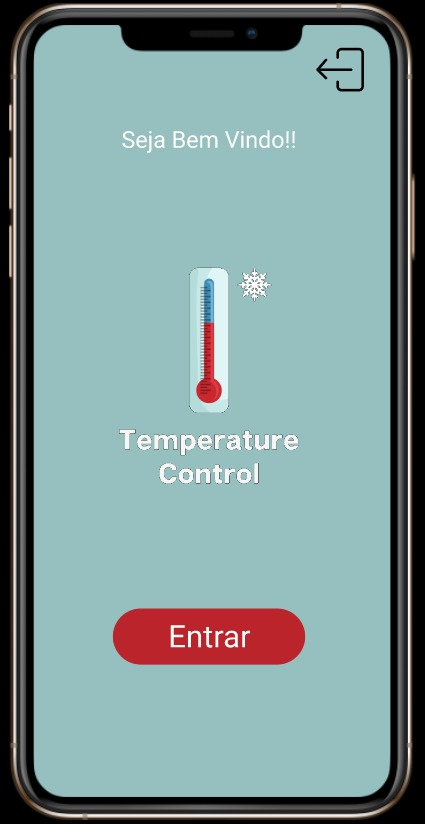
\includegraphics[scale=0.5]{img/mobile/bem_vindo.png}
        \legend{Fonte: Elaborado pelos autores}
        \label{fig:mobileBemVindo}
    \end{figure}

    \begin{figure}[ht]
        \caption{Layout mobile Home}
        \centering
        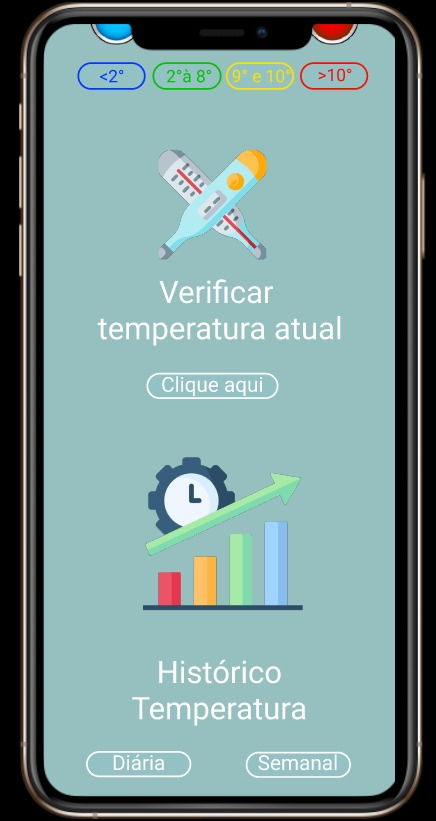
\includegraphics[scale=0.5]{img/mobile/home.jpeg}
        \legend{Fonte: Elaborado pelos autores}
        \label{fig:mobileHome}
    \end{figure}

    \begin{figure}[ht]
        \caption{Layout mobile configuração temperaturas}
        \centering
        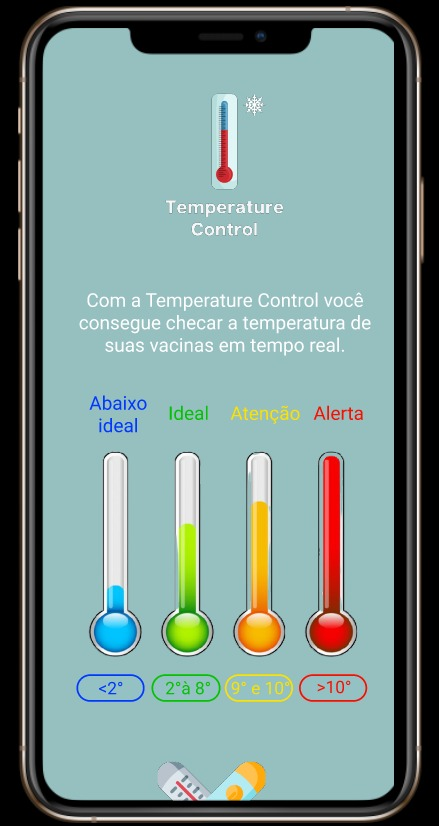
\includegraphics[scale=0.5]{img/mobile/config_temp.jpeg}
        \legend{Fonte: Elaborado pelos autores}
        \label{fig:mobileConfig}
    \end{figure}

    \begin{figure}[ht]
        \caption{Layout mobile dashboard 1}
        \centering
        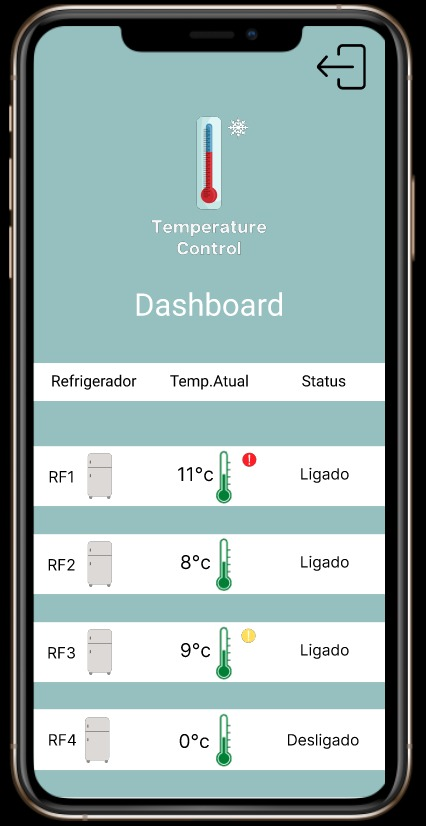
\includegraphics[scale=0.5]{img/mobile/dashboard_1.jpeg}
        \legend{Fonte: Elaborado pelos autores}
        \label{fig:mobileDashboard1}
    \end{figure}

    \begin{figure}[ht]
        \caption{Layout mobile dashboard 2}
        \centering
        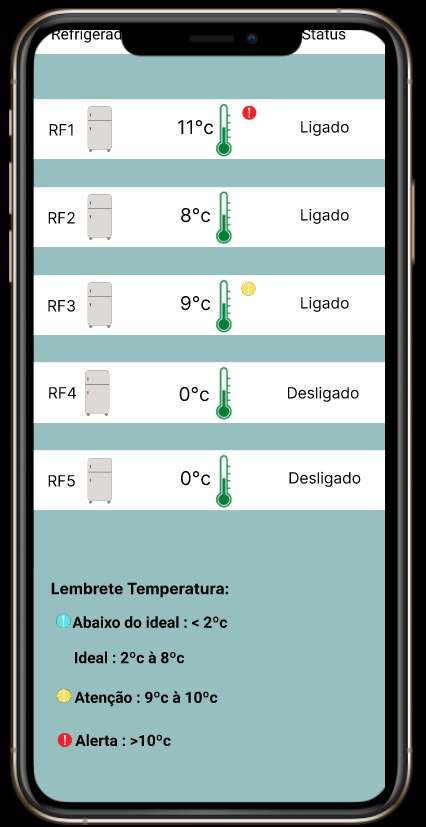
\includegraphics[scale=0.5]{img/mobile/dashboard_2.jpeg}
        \legend{Fonte: Elaborado pelos autores}
        \label{fig:mobileDashboard2}
    \end{figure}

    \begin{figure}[ht]
        \caption{Layout mobile temperatura atual}
        \centering
        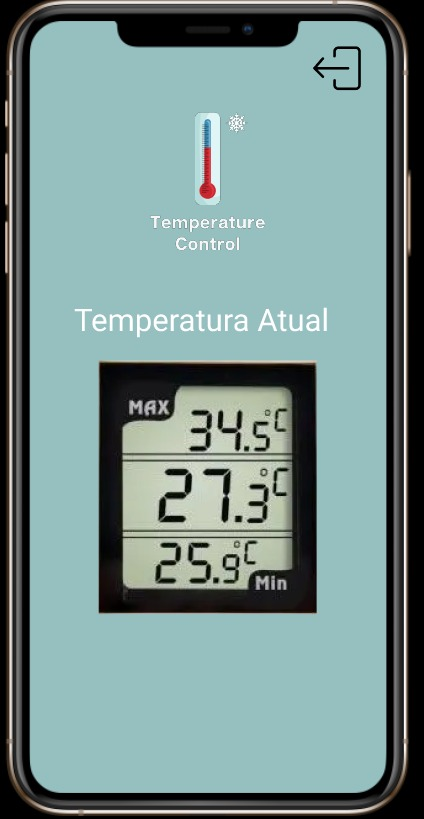
\includegraphics[scale=0.5]{img/mobile/temp_atual.jpeg}
        \legend{Fonte: Elaborado pelos autores}
        \label{fig:mobileTempAtual}
    \end{figure}

    \begin{figure}[ht]
        \caption{Layout mobile histórico diário}
        \centering
        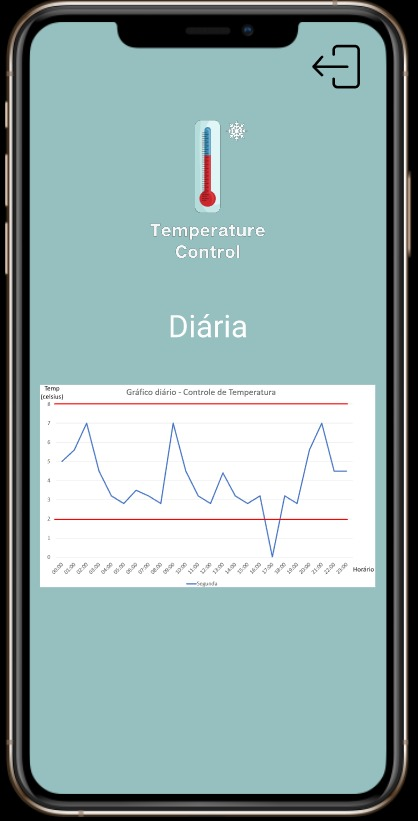
\includegraphics[scale=0.5]{img/mobile/temp_diaria.jpeg}
        \legend{Fonte: Elaborado pelos autores}
        \label{fig:mobileTempDiaria}
    \end{figure}

    \begin{figure}[ht]
        \caption{Layout mobile histórico semanal}
        \centering
        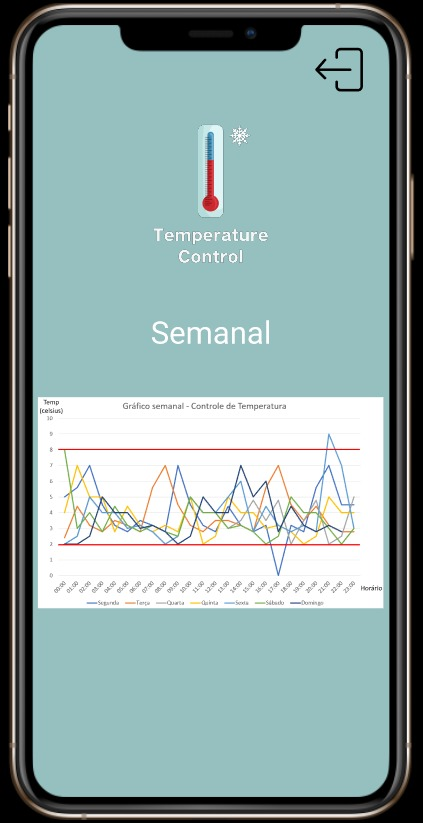
\includegraphics[scale=0.5]{img/mobile/temp_semanal.jpeg}
        \legend{Fonte: Elaborado pelos autores}
        \label{fig:mobileTempSemanal}
    \end{figure}


    % \begin{figure}[htb!]
        % \caption{Tela inicial do sistema}
        % \centering
        % 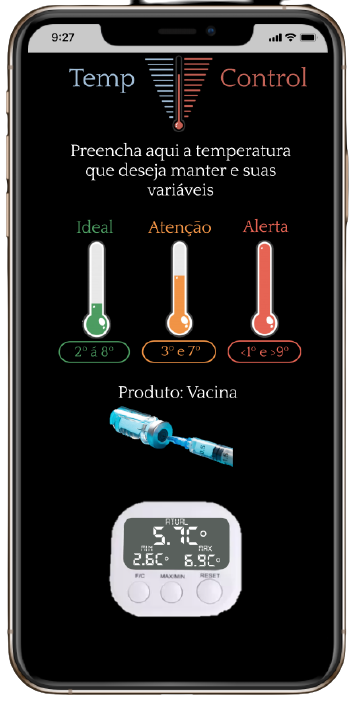
\includegraphics[scale=0.5]{img/sistema_home.png}
        % \legend{Fonte: Elaborado pelos autores}
        % \label{fig:sistemaHome}
    % \end{figure}
%
    % \begin{figure}[ht]
        % \caption{Tela de histórico de temperatura}
        % \centering
        % 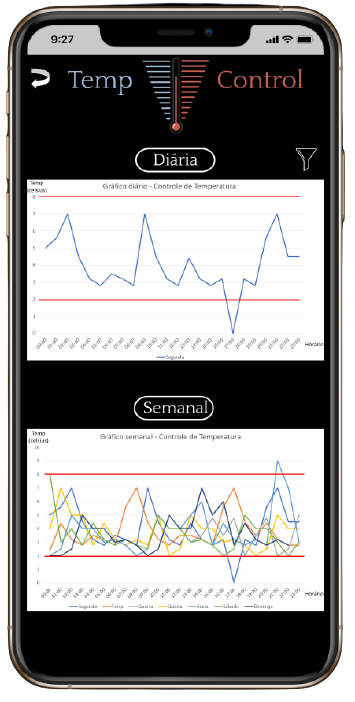
\includegraphics[scale=0.4]{img/sistema_historico.png}
        % \legend{Fonte: Elaborado pelos autores}
        % \label{fig:sistemaHistorico}
    % \end{figure}
%
    % \begin{figure}[t]
        % \caption{Tela de visualização em tempo real}
        % \centering
        % 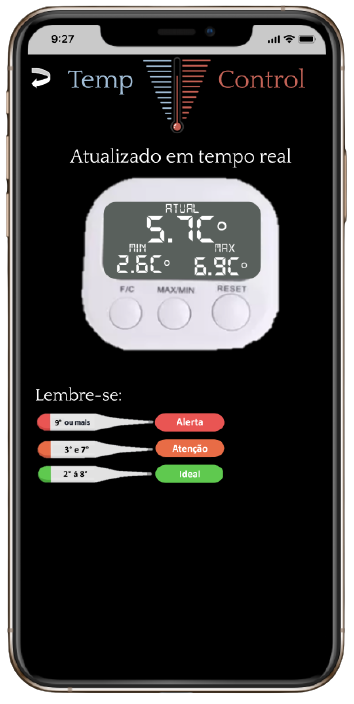
\includegraphics[scale=0.4]{img/sistema_temp_real.png}
        % \legend{Fonte: Elaborado pelos autores}
        % \label{fig:sistemaTempReal}
    % \end{figure}
%

    \begin{figure}[ht]
        \caption{Layout desktop home}
        \centering
        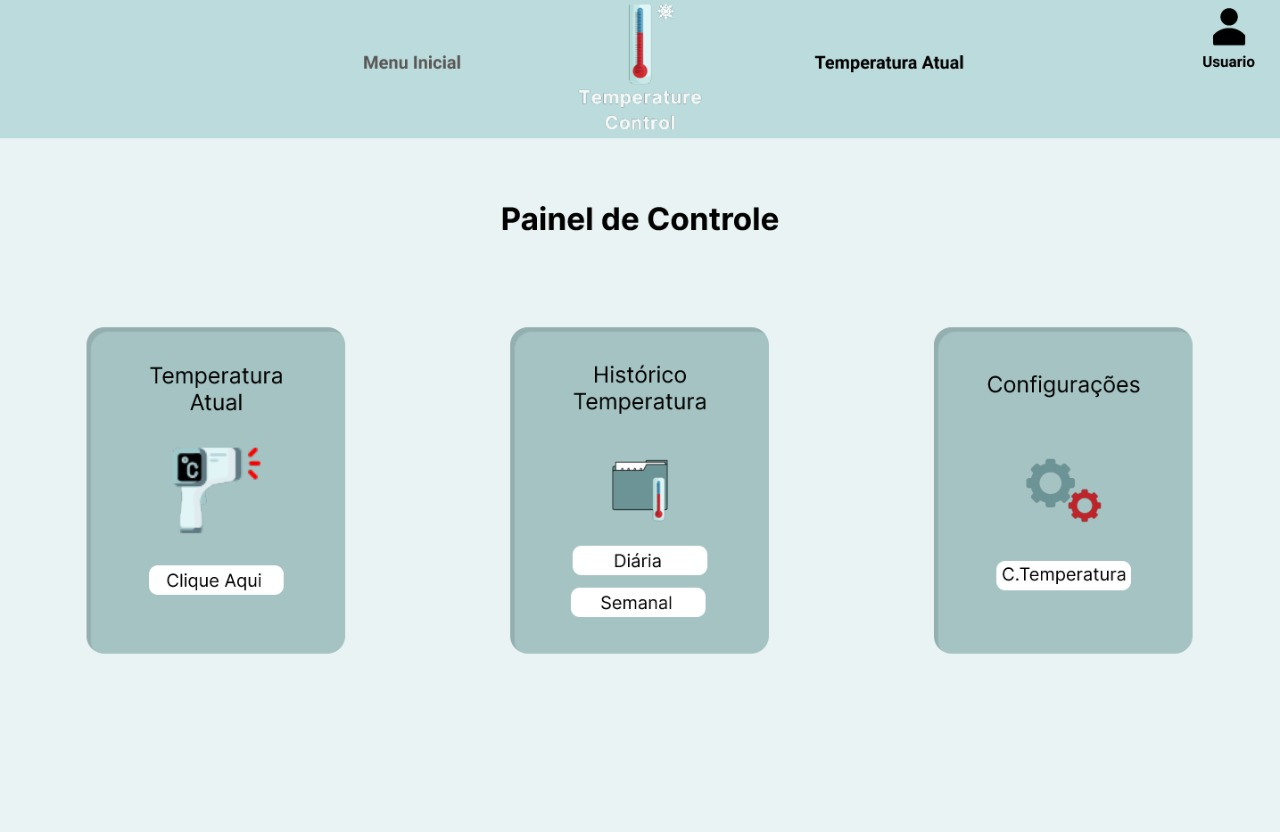
\includegraphics[scale=0.35]{img/desktop/home.jpeg}
        \legend{Fonte: Elaborado pelos autores}
        \label{fig:desktopHome}
    \end{figure}

    \begin{figure}[ht]
        \caption{Layout desktop configuração de temperatura}
        \centering
        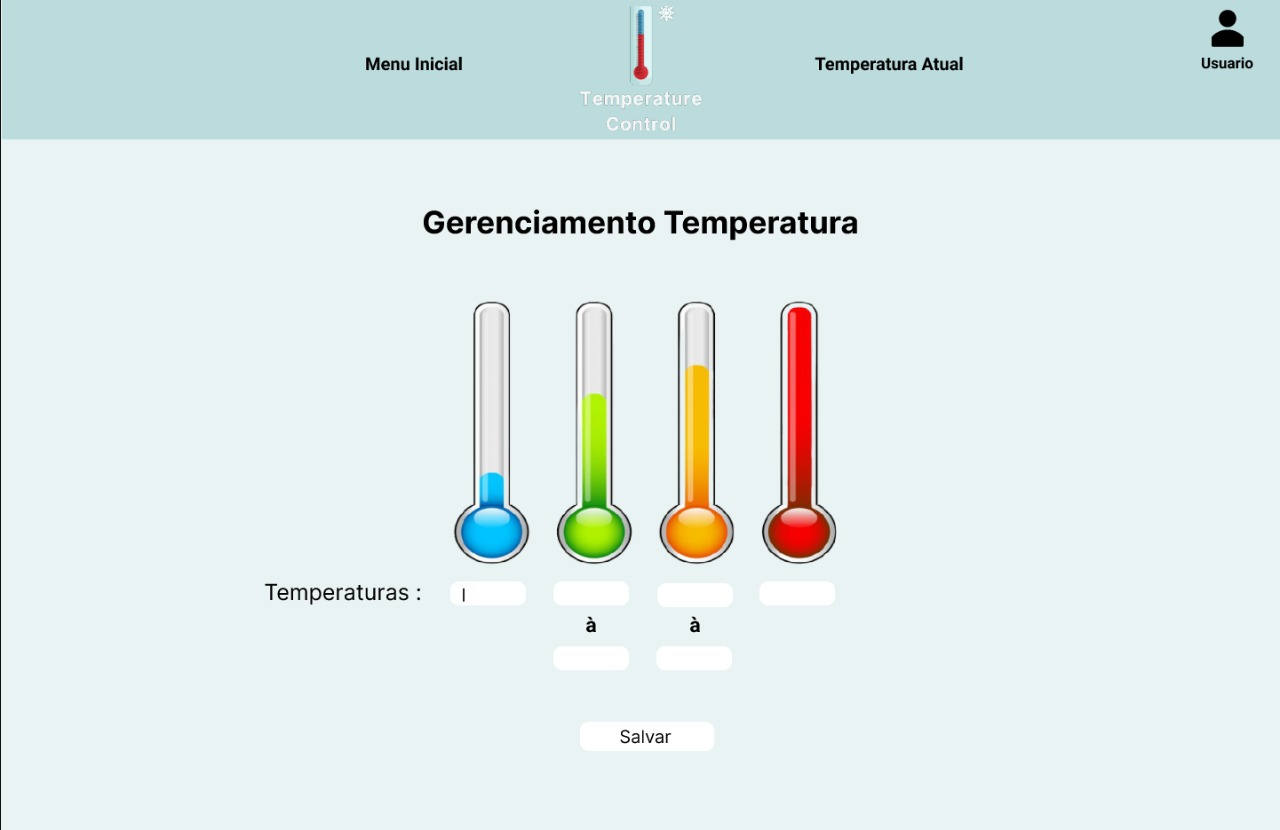
\includegraphics[scale=0.35]{img/desktop/config_temp.jpeg}
        \legend{Fonte: Elaborado pelos autores}
        \label{fig:desktopConfigTemp}
    \end{figure}

    \begin{figure}[ht]
        \caption{Layout desktop temperatura atual}
        \centering
        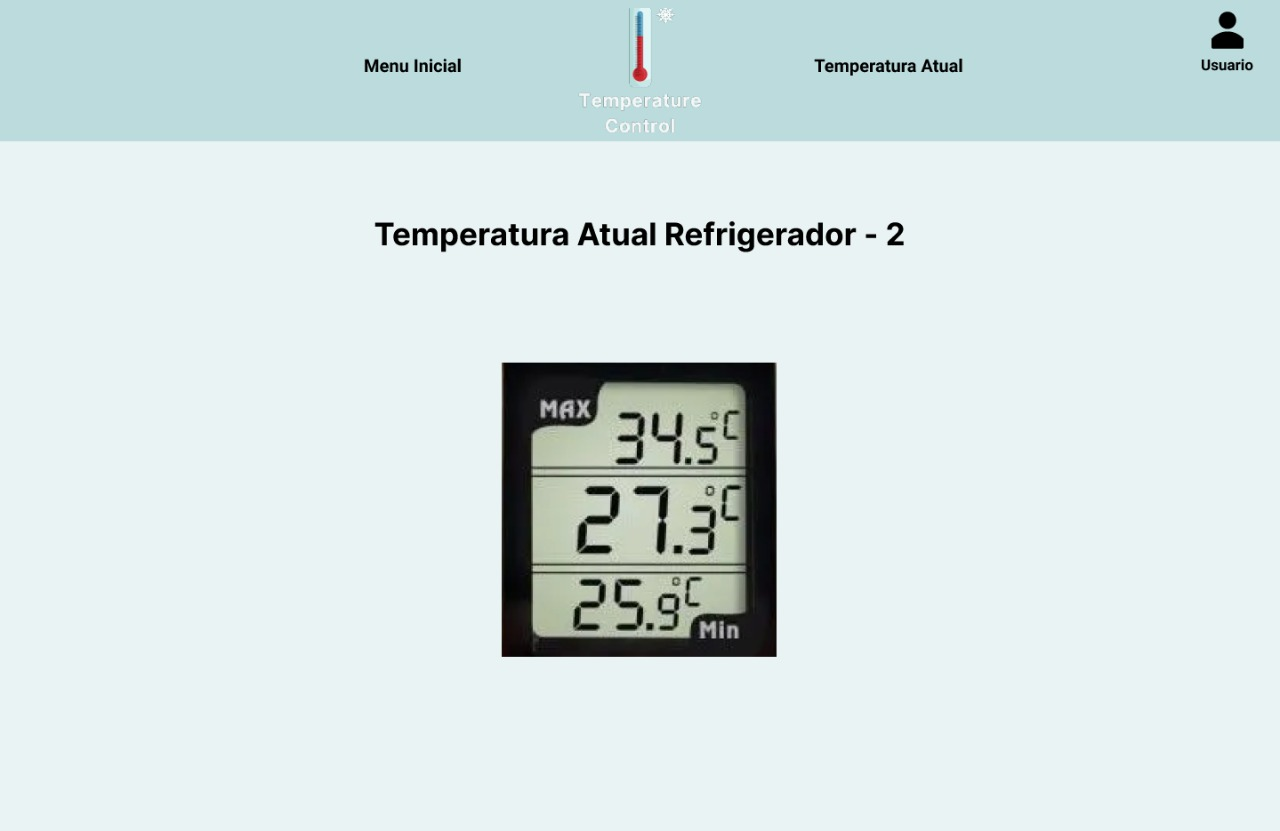
\includegraphics[scale=0.35]{img/desktop/temp_atual.jpeg}
        \legend{Fonte: Elaborado pelos autores}
        \label{fig:desktopTempAtual}
    \end{figure}

    \begin{figure}[ht]
        \caption{Layout desktop dashboard 1}
        \centering
        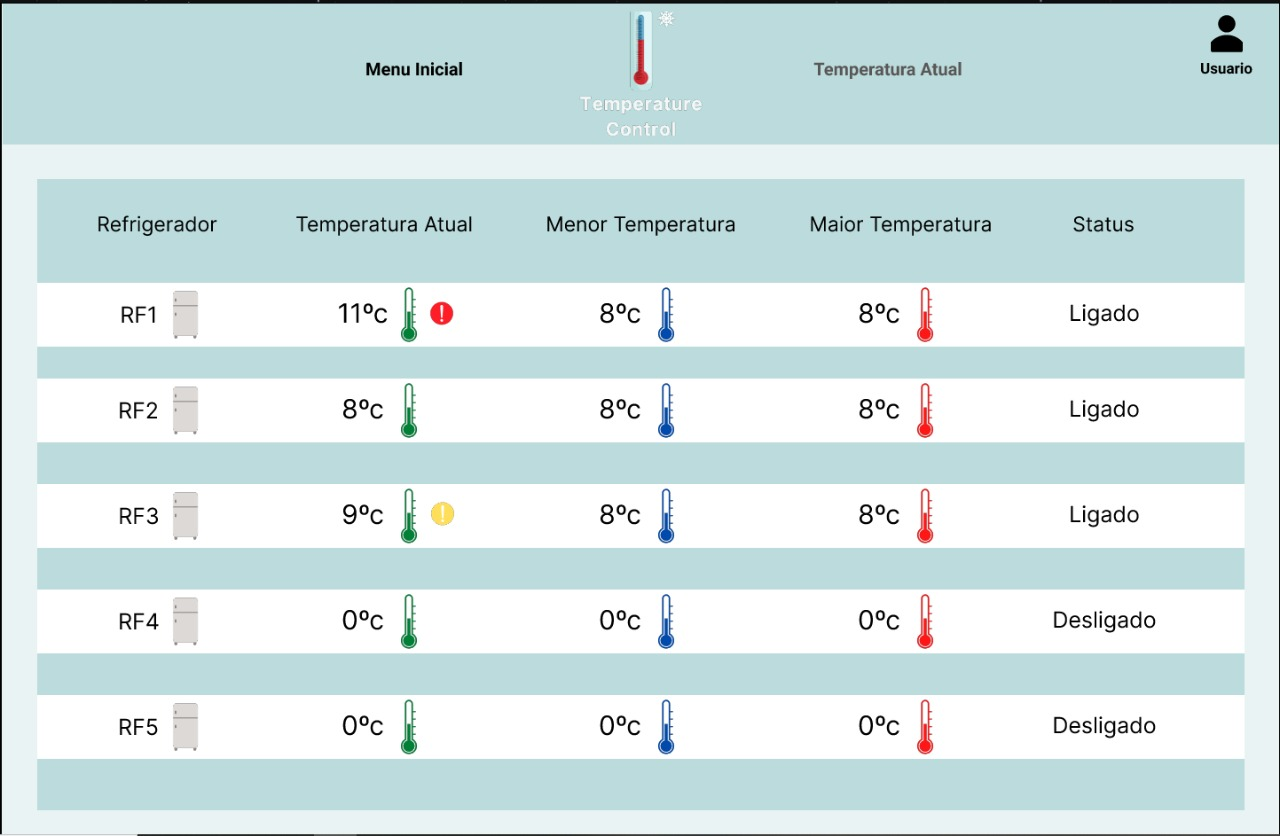
\includegraphics[scale=0.35]{img/desktop/dashboard_1.jpeg}
        \legend{Fonte: Elaborado pelos autores}
        \label{fig:desktopDashboard1}
    \end{figure}

    \begin{figure}[ht]
        \caption{Layout desktop dashboard 2}
        \centering
        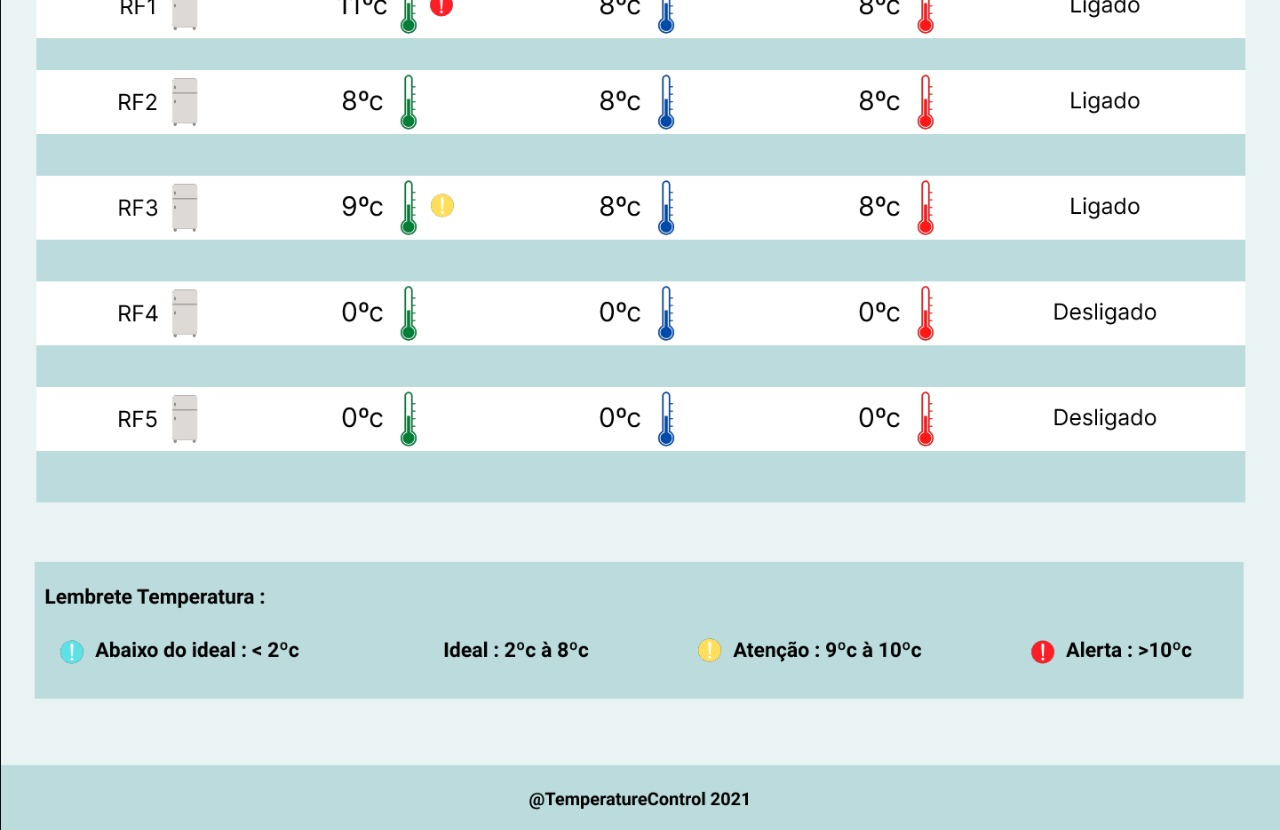
\includegraphics[scale=0.35]{img/desktop/dashboard_2.jpeg}
        \legend{Fonte: Elaborado pelos autores}
        \label{fig:desktopDashboard2}
    \end{figure}

    \begin{figure}[ht]
        \caption{Layout desktop histórico diário}
        \centering
        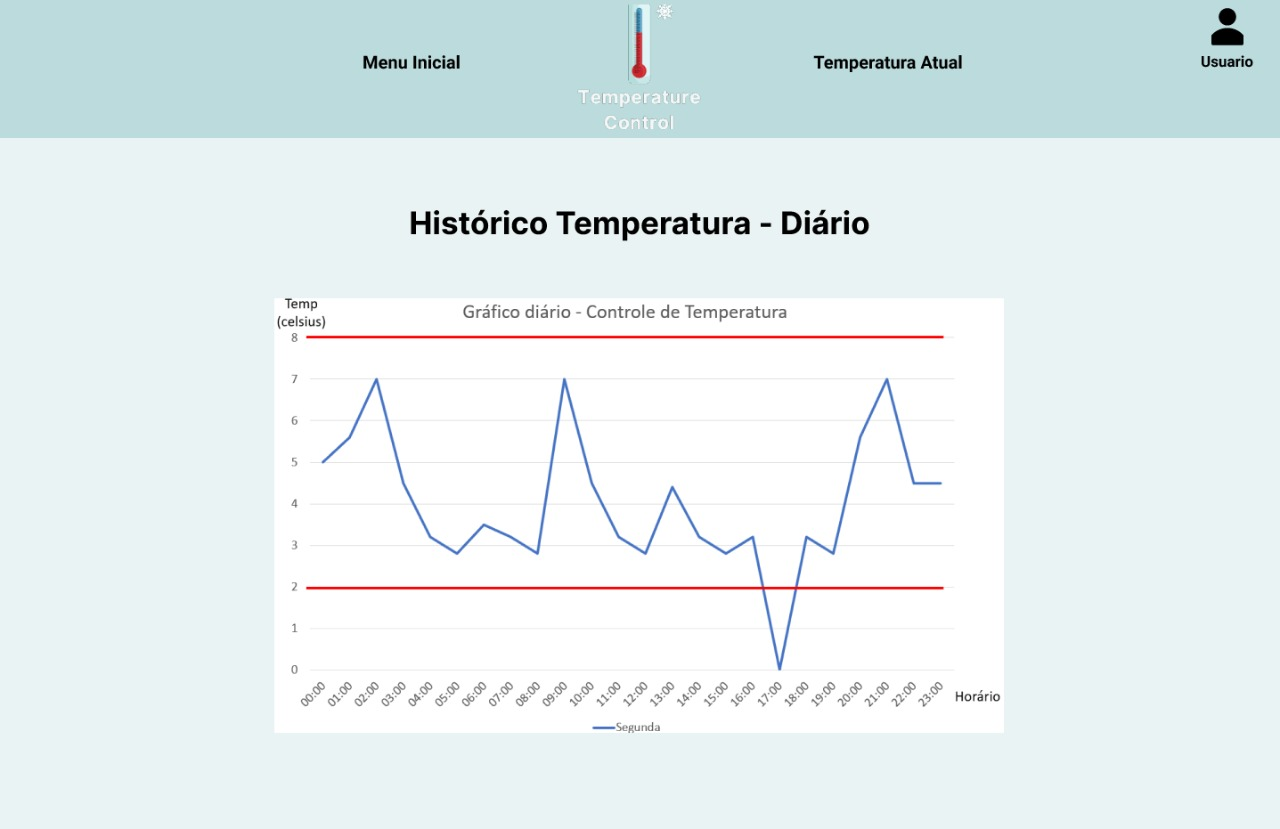
\includegraphics[scale=0.35]{img/desktop/temp_diaria.jpeg}
        \legend{Fonte: Elaborado pelos autores}
        \label{fig:desktopTempDiaria}
    \end{figure}

    \begin{figure}[ht]
        \caption{Layout desktop histórico semanal}
        \centering
        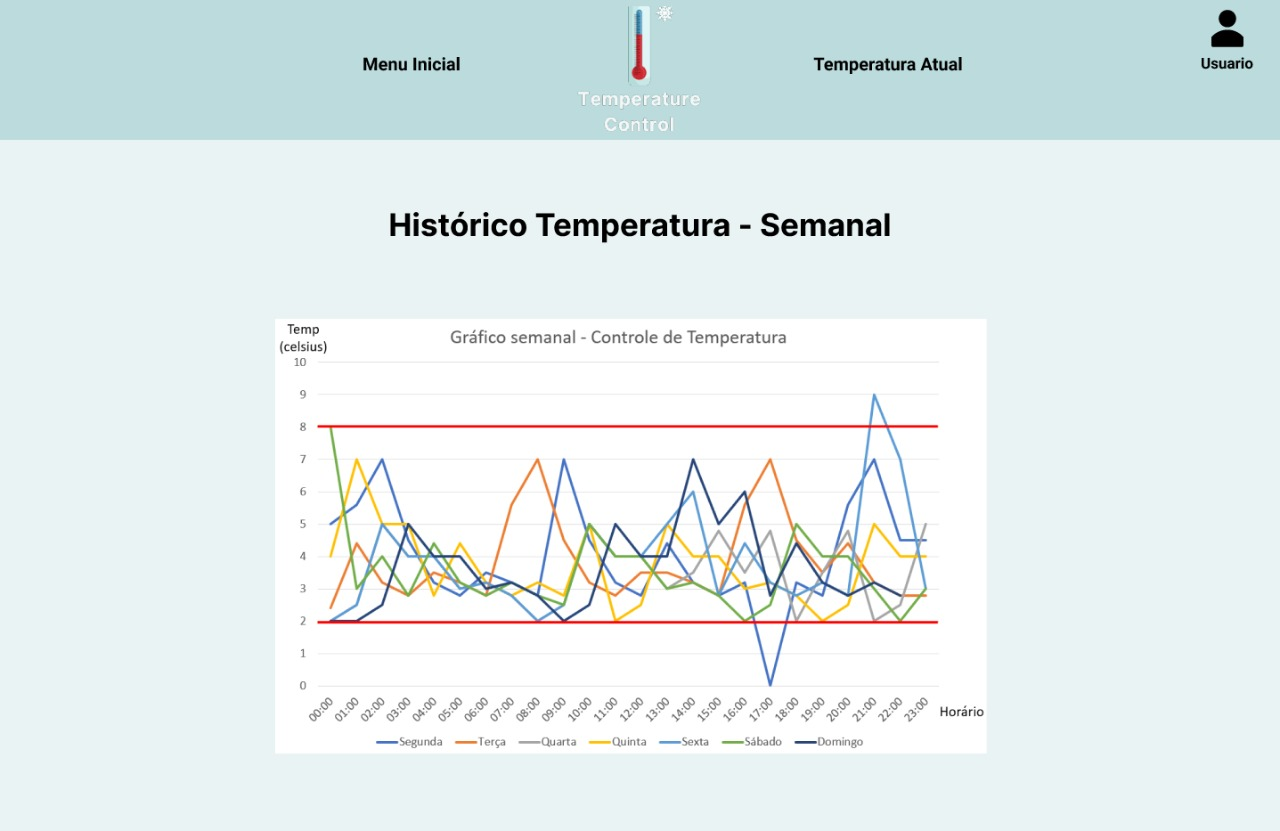
\includegraphics[scale=0.35]{img/desktop/temp_semanal.jpeg}
        \legend{Fonte: Elaborado pelos autores}
        \label{fig:desktopTempSemanal}
    \end{figure}
